%%=============================================================================
%% Methodologie
%%=============================================================================

\chapter{\IfLanguageName{dutch}{Methodologie}{Methodology}}%
\label{ch:methodologie}

%% TODO: In dit hoofstuk geef je een korte toelichting over hoe je te werk bent
%% gegaan. Verdeel je onderzoek in grote fasen, en licht in elke fase toe wat
%% de doelstelling was, welke deliverables daar uit gekomen zijn, en welke
%% onderzoeksmethoden je daarbij toegepast hebt. Verantwoord waarom je
%% op deze manier te werk gegaan bent.
%% 
%% Voorbeelden van zulke fasen zijn: literatuurstudie, opstellen van een
%% requirements-analyse, opstellen long-list (bij vergelijkende studie),
%% selectie van geschikte tools (bij vergelijkende studie, "short-list"),
%% opzetten testopstelling/PoC, uitvoeren testen en verzamelen
%% van resultaten, analyse van resultaten, ...
%%
%% !!!!! LET OP !!!!!
%%
%% Het is uitdrukkelijk NIET de bedoeling dat je het grootste deel van de corpus
%% van je bachelorproef in dit hoofstuk verwerkt! Dit hoofdstuk is eerder een
%% kort overzicht van je plan van aanpak.
%%
%% Maak voor elke fase (behalve het literatuuronderzoek) een NIEUW HOOFDSTUK aan
%% en geef het een gepaste titel.

Volgende hoofdstukken verlopen in sequentiële volgorde om dit onderzoek in de juiste richting te sturen.
De literatuurstudie geeft een basis om verdere vakterminologie en de werking van technologieën te kunnen begrijpen.
\\
De opzet van het huidige systeem wordt besproken om de requirements te kunnen begrijpen.
Het bekomen van een shortlist wordt toegelicht waarbij voor elke technologie de voor- en nadelen wordt beschreven.

\section{Phase 1: Literatuurstudie}
Voor dit onderzoek werden de vaktermen opgesomd en onderverdeeld in groepen met behulp van een mindmap.
Vervolgens werd er gebruik gemaakt van het internet om wetenschappelijke artikelen op te zoeken om de nodige informatie uit te filteren.
\\
Het doel van de literatuurstudie is om een basis van bestaande kennis te verkrijgen door de belangrijkste concepten toe te lichten die van toepassing zijn op dit onderzoek. 
Dit houdt in, het begrijpen van warehousing, WCS (Warehouse Control Systems), PLC (Programmable Logic Controllers), en de communicatieprotocollen die tussen deze systemen gebruikt worden.
\\
Hierdoor krijg je een overzicht van relevante theorieën, definities, en eerdere studies die inzicht geven in de werking en de gebruikte technologieën.
Er werd voornamelijk gebruik gemaakt van wetenschappelijke artikelen, boeken en technische documenten.
\\
De literatuurstudie vormt de basis van het onderzoek en is cruciaal voor het begrijpen van de huidige stand van zaken.
Hierdoor kan de kennis en vereisten meegenomen worden doorheen de methodologie.

\section{Phase 2: Long List}
Dit hoofdstuk vertrekt vanuit een lijst met message brokers die beschikbaar zijn op de markt.
Deze worden later gefilterd door bepaalde criteria toe te passen, waarna de overgebleven kandidaten getest kunnen worden.
Op deze manier worden alle mogelijke opties geargumenteerd.

\subsection{Beschikbare messaging software}
Deze lijst bevat relevante message brokers als startpunt die beschikbaar zijn op de markt.
Bronnen werden geraadpleegd via zoekmachines, forums en blogs.

\begin{table}[!h]
\footnotesize
\centering
\begin{tabular}{|l|c|c|c|c|c|}
\hline
Message Broker & JMS & Linux & Protocollen & Kostenmodel & On premise \\
\hline
Apache Kafka & Ja & Ja & Kafka, MQTT, REST & Open-source & Ja \\
\hline
RabbitMQ & Ja & Ja & AMQP, MQTT, STOMP & Open-source & Ja \\
\hline
ActiveMQ & Ja & Ja & AMQP, MQTT, STOMP, OpenWire & Open-source & Ja \\ 
\hline
Artemis & Ja & Ja & AMQP, MQTT, STOMP & Open-source & Ja \\
\hline
MQTT.js & Ja & Ja & MQTT & Open-source & Ja \\
\hline
IBM MQ & Ja & Ja & MQ, MQTT & Abonnement & Ja \\
\hline
Redis & Ja & Ja & Stream, Pub/Sub & Open-source & Ja \\
\hline
NSQ & Ja & Ja & Stream, Pub/Sub & Open-source & Ja \\
\hline
Apache Pulsar & Ja & Ja & Stream, Pub/Sub & Open-source & Ja \\
\hline
NATS & Ja & Ja & NATS & Open-source & Ja \\
\hline
ZeroMQ & Ja & Ja & ØMQ (Socket) & Open-source & Ja \\ 
\hline
Amazon SQS & Nee & Nee & AWS protocol & Pay-per-use & Nee \\
\hline
Google Cloud Pub/Sub & Nee & Nee & Cloud Pub/Sub & Pay-per-use & Nee \\
\hline
Azure Service Bus & Nee & Nee & AMQP, MQTT, HTTP & Pay-per-use & Nee \\
\hline
Solace PubSub+ & Ja & Nee & AMQP & Pay-per-use & Nee \\
\hline
\end{tabular}
\caption{\label{tab:message_brokers}Longlist message brokers}
\end{table}

\section{Phase 3: Requirements analyse van huidige setup}
Dit hoofdstuk gaat dieper in op de huidige setup en werking tussen het WCS, messaging software en de PLC's.
Documenten van het bedrijf en interviews met vakexperts vormen de basis voor dit overzicht.
\\
Het doel is om na het lezen van dit hoofdstuk inzicht te krijgen in de requirements van het huidige systeem, 
zodat deze kunnen dienen als basis voor de keuze van een surrogaat voor het huidige messaging systeem.

\subsection{PLC gebruik binnen TVH}
Er zijn 7 verschillende PLC's in TVH Waregem die instaan voor verschillende zones van de conveyor.
Deze werden aangeleverd door Vanderlanden in het jaar 2013 en worden beheerd door het automatisatieteam.
De communicatie tussen een PLC en het WCS is gebaseerd op het TCP/IP-protocol en is verbonden via het intern netwerk.
Er is een tussenlaag tussen de PLC en het netwerk, RFC1006 van het merk Siemens waarin configuratie kan worden gedaan door het automatisatie team.
Dit stelt de collega's in staat om bepaalde logica te implementeren of netwerk aanpassingen door te voeren.
De snelheid van communicatie is essentieel, daarom moet het netwerk snel genoeg zijn zodat berichten aan een snel tempo verstuurd kunnen worden.
\\\\
De PLC's maken gebruik van een TCP/IP-socketverbinding en functioneren als client ten opzichte van het WCS, dat de rol van server vervult. 
Dit betekent dat de PLC de verbinding initieert en persisteert met de server die verantwoordelijk is voor de communicatie.
Een PLC is verantwoordelijk voor een specifieke zone van de conveyor en is opgebouwd uit drie kanalen die elk via een toegewezen poortnummer met de server communiceren. 
Meerdere kanalen zijn nodig om de communicatiesnelheid te bevorderen en omdat elk kanaal zijn eigen type informatie verwerkt.

\begin{table}[!h]
  \centering
  \begin{tabular}{lcr}
    \toprule
    \textbf{Kanaal} & \textbf{Beschrijving} & \textbf{Type}                        \\
    \midrule
    1                & Route informatie over transportbak          & Snel           \\
    2                & Informatie van PLC                          & Niet kritisch  \\
    3                & Overige informatie over transportbak        & Snel           \\
    \bottomrule
  \end{tabular}
  \caption[Channel assignment]{\label{tab:channel-assignment}Beschrijving van kanalen}
\end{table}

\subsubsection{PLC berichten}
Berichten bestaan uit een frame opgedeeld in velden en hebben een specifieke lengte.
De inhoud van een bericht is gebaseerd op het hexadecimale stelsel en wordt in detail toegelicht in de onderstaande tabel.
\begin{table}[h!]
\centering 
\begin{tabular}{|c|c|c|c|}
  \hline
  \textbf{Veld} & \textbf{Inhoud} & \textbf{Data type} & \textbf{Lengte} \\
  % \hline
  % Dummy & Enkel PLC naar WCS
  \hline 
  Header & <STX> & Binair & 1 byte \\
  \hline 
  Lengte in bytes & 001D(HEX) & Binair & 2 bytes \\
  \hline 
  Seq. nummer &  [0-9] & ASCII & 1 byte  \\
  \hline 
  Inhoud & <...> & Binair & 27 bytes \\
  \hline 
  Terminator & <ETX> & Binair & 1 byte \\
  \hline
\end{tabular}
\caption[Message content]{\label{tab:message-content}Inhoud bericht}
\end{table}

Bepaalde controles worden uitgevoerd om de validiteit van een bericht af te toetsen. 
\\\\
Er worden ongeveer 80 berichten per minuut verstuurd per PLC, per kanaal.
Het totale aantal verstuurde berichten per minuut komt uit op ongeveer 1680/min.

Voorbeeld van een bericht dat van PLC naar WCS wordt verstuurd: 
\begin{listing}[h!]
\begin{minted}{python}
  02 00 1d 20 30 36 20 20 00 00 20 20 30 37 20 20 30 20 20 20 20 20 20 20 20 20 20 20 20 20 20 03
\end{minted}
\caption[Voorbeeld PLC bericht]{\label{listing:message_example}Voorbeeld van een PLC bericht}
\end{listing}

\subsection{Java listeners}
De PLC kan uitsluitend maar een TCP/IP-socket verbinding initiëren met een server.
Omdat SonicMQ als middleware hierdoor geen verbinding kan maken zijn er Java-listeners gemaakt door TVH.
Deze listeners fungeren als server en zijn specifiek opgesteld om een TCP/IP-socket verbinding mogelijk te maken per PLC kanaal.
De Java-listeners sturen de PLC-berichten vervolgens door naar SonicMQ of ontvangen berichten van SonicMQ, 
die ze via een socket naar de PLC doorsturen.
Aan de kant van het WCS zijn er meer mogelijkheden om verbinding te kunnen maken met een server.
SonicMQ biedt geen support meer en is niet populair waardoor er ook geen community is.
Dit kan leiden tot extra kosten of langdurige problemen.

\subsection{WCS communicatie} 
Op het ERP-systeem van TVH draaien acht verschillende batches die verantwoordelijk zijn voor de aansturing van de PLC. 
Elke batch-instantie communiceert met specifieke PLC-kanalen en bevat daarvoor specifieke logica, geschreven in OpenEdge Progress 4GL.
Deze batches zijn verbonden via een specifieke poort met een \textbf{Progress JMS Adapter} op de communicatieserver omdat ze de ``Broker connect'' methode gebruiken.
Hiermee kunnen de batches de berichten consumeren en versturen van de SonicMQ server.
Daarnaast is het ook mogelijk om de Client connect methode te gebruiken, wat gemakkelijker is qua integratie.

\subsubsection{Progress OpenEdge JMS Adapter}
De adapter stelt OpenEdge-applicaties in staat om berichten te verzenden en te ontvangen van JMS (Java Messaging System)
messagebrokers zoals Apache ActiveMQ. 
Dit betekent dat OpenEdge-applicaties kunnen integreren met andere systemen die JMS ondersteunen, 
zonder dat er directe afhankelijkheden nodig zijn.
Hierdoor is de keuze van message brokers gelimiteerd tot brokers die \textbf{JMS ondersteunen}.

\subsubsection{Integratie met Verschillende Enterprise Systemen}
Met de JMS Adapter kunnen OpenEdge-applicaties communiceren met andere systemen zoals ERP en CRM-systemen, 
wat nuttig is in bedrijfsprocessen waarbij gegevens moeten worden gedeeld tussen verschillende systemen.

\subsubsection{Configuratie en Beheer}
De Progress OpenEdge JMS Adapter biedt configuratiemogelijkheden waarmee beheerders de communicatie kunnen aanpassen 
aan de vereisten van hun omgeving, zoals het instellen van queue-namen, topics, verbindingsparameters, en het beheren van uitzonderingen.

\subsubsection{WCS berichten} 
Berichten komen binnen van de PLC via de communicatie server. Ieder bericht wordt getransformeerd naar variabelen die dan verder gebruikt worden in de code.
Deze berichten bevatten informatie over transportbakken en zijn nodig om deze te kunnen traceren via de ERP.
Specifieke logica is nodig om bakken tot hun bestemming te krijgen, of om fout afhandeling te voorzien.
\\\\
Volgende voorbeelden doen zich voor:
\begin{enumerate}
\item Routeren naar een hospitaal punt door: 
\begin{enumerate}
  \item Gewichtsfout
  \item Hoogtefout
  \item Onbekende bestemming
\end{enumerate}
\item Bestemming wordt gevraagd door de PLC
\item Bestemming wordt doorgegeven aan de PLC 
\item Specifieke logica moet uitgevoerd worden bij het passeren van een bepaald punt
\item \dots
\end{enumerate}

\subsection{Monitoring}
Het bestaande systeem wordt visueel gemonitord met behulp van Grafana en Elastic. 
Voor het ophalen van de logging wordt gebruik gemaakt van Prometheus.
Hierdoor kunnen systeemfouten snel opgemerkt worden en berichten verstuurd worden als bepaalde waardes overschreden worden.
\newpage

\subsection{Samenvatting requirements messaging systeem}
De belangrijkste requirements voor de huidige setup zijn als volgt:

\subsubsection{Integratie met het WCS systeem}
Het messaging systeem moet kunnen integreren met het huidige WCS-systeem dat gebruik maakt van Progress 4GL versie 11.7. 
Hiervoor moet de broker het \textbf{JMS protocol ondersteunen} en geïnstalleerd kunnen worden op een \textbf{Linux platform}.
Daarnaast moet de middleware ook gebruikt kunnen worden door \textbf{monitoring software}.

\subsubsection{Performantie}
Om de real-time eisen van het WCS en de PLC’s te ondersteunen, moet het messaging systeem \textbf{hoge performantie} bieden. 
Dit betekent dat berichten zonder merkbare vertraging moeten worden verstuurd en ontvangen, 
zodat de snelheid van de conveyor niet wordt beperkt door de communicatiesnelheid.
Om vertraging te voorkomen moet de verwerking van de berichten \textbf{asynchroon} gebeuren.

\subsubsection{Betrouwbare Berichtenoverdracht}
Het systeem moet in staat zijn berichten \textbf{consistent, sequentieel en zonder verlies} over te brengen. 
Dit is essentieel om de traceerbaarheid van transportbakken te garanderen en fouten in de logistieke processen te voorkomen.
Hiervoor moet de broker het \textbf{AMQP-protocol} ondersteunen.

\subsubsection{Support en Community}
Het is belangrijk dat de gekozen message broker support biedt en dat er een grote community aanwezig is 
waarbij je terecht kunt voor advies, probleemoplossing en best practices.
Daarnaast is het ook belangrijk dat er commerciële support beschikbaar is om SLA's (Service Level Agreement's) te kunnen afdwingen.

\subsubsection{Kosten}
Support gaat vaak samen met kosten en is ook belangrijk om mee te nemen in de keuze van een messaging systeem.
Sommige systemen hangen vast aan een kostenmodel, andere zijn \textbf{open-source} en zijn kosteloos.
\newpage
\subsubsection{MoSCoW prioriteiten}

\textbf{Must have:}
\begin{itemize}
\item Hoge performantie 
\item Asynchroon verzenden van gegevens  
\item JMS ondersteuning
\item Installatie mogelijk op Linux OS 
\item AMQP-protocol ondersteunen 
\item Monitoring mogelijkheden
\item Moet lokaal kunnen geïnstalleerd worden
\item Commerciële support
\end{itemize}

\textbf{Should have:}
\begin{itemize}
  \item Kostenmodel: open source 
  \item Uitgebreide documentatie
  \item Gemakkelijk op te schalen: om niet beperkt te worden in groei
  \item Gebruiksvriendlijkheid
\end{itemize}

\textbf{Could have}:
\begin{itemize}
  \item Actieve Community en support
  \item UI console via web pagina 
  \item Filtering op properties
\end{itemize}

\newpage
\section{Phase 5: ShortList}
In deze sectie worden de message brokers uit de longlist opgelijst en stapsgewijs gefilterd op basis van het MoSCoW principe.
Het doel is om een top 3 te bekomen waarbij uitvoerige testen kunnen uitgevoerd worden.

\subsection{Must have}
In deze sectie wordt de longlist van beschikbare messaging brokers gefilterd op basis van de gestelde must-have criteria. 
Messaging brokers die niet voldoen aan een van deze criteria worden verworpen, omdat de must-have eisen de hoogste prioriteit hebben.
\\\\
Voor elke technologie wordt een onderbouwde argumentatie gegeven op basis van de must-have criteria om de gemaakte keuzes inzichtelijk te maken. 
Het aspect van hoge prestaties, dat eveneens onderdeel is van de must-have criteria, wordt geëvalueerd tijdens de testen.
\\\\
Producten die voldoen aan de ``must-have'' criteria worden als kandidaat gemarkeerd en meegenomen naar de volgende stap, waarin ``should-have'' criteria worden toegepast.
 
\subsubsection{Apache Kafka}
\textbf{Pro:}
\begin{itemize}
    \item Hoge prestaties bij grote hoeveelheden gegevens.
    \item Volledige asynchrone verwerking.
    \item Uitgebreide monitoringmogelijkheden.
    \item Lokaal te installeren.
    \item Beschikbaarheid van commerciële ondersteuning.
\end{itemize}
\textbf{Con:}
\begin{itemize}
    \item Geen native AMQP-ondersteuning.
    \item Geen native JMS-ondersteuning.
    \item Niet volledig compatibel met huidige setup.
\end{itemize}

\subsubsection{RabbitMQ}
\textbf{Pro:}
\begin{itemize}
    \item Hoge prestaties en efficiëntie.
    \item Volledige asynchrone verwerking.
    \item Ondersteunt AMQP en JMS.
    \item Uitgebreide monitoringmogelijkheden.
    \item Lokaal te installeren.
    \item Beschikbaarheid van commerciële ondersteuning.
\end{itemize}
\textbf{Con:}
\begin{itemize}
    \item Geen significante nadelen gevonden binnen de gestelde vereisten.
\end{itemize}

\subsubsection{ActiveMQ Classic}
\textbf{Pro:}
\begin{itemize}
    \item Goede prestaties.
    \item Ondersteunt AMQP en JMS.
    \item Uitgebreide monitoringmogelijkheden.
    \item Lokaal te installeren.
    \item Beschikbaar zonder licentiekosten.
\end{itemize}
\textbf{Con:}
\begin{itemize}
    \item Verminderde focus van community op Classic-versie.
\end{itemize}

\subsubsection{ActiveMQ Artemis}
\textbf{Pro:}
\begin{itemize}
    \item Hoge prestaties met geoptimaliseerde architectuur.
    \item Ondersteunt AMQP en JMS.
    \item Uitgebreide monitoringmogelijkheden.
    \item Lokaal te installeren.
    \item Beschikbaarheid van commerciële ondersteuning.
\end{itemize}
\textbf{Con:}
\begin{itemize}
    \item Geen significante nadelen gevonden binnen de gestelde vereisten.
\end{itemize}

\subsubsection{MQTT.js}
\textbf{Pro:}
\begin{itemize}
    \item Uitstekende prestaties voor MQTT-protocol.
    \item Volledig asynchrone verwerking.
    \item Lokaal te installeren in Node.js-omgeving.
\end{itemize}
\textbf{Con:}
\begin{itemize}
    \item Geen ondersteuning voor JMS en AMQP.
    \item Beperkte monitoringmogelijkheden.
    \item Geen commerciële ondersteuning.
\end{itemize}

\subsubsection{IBM MQ}
\textbf{Pro:}
\begin{itemize}
    \item Hoge prestaties met enterprise-grade betrouwbaarheid.
    \item Ondersteunt AMQP en JMS.
    \item Uitgebreide monitoringmogelijkheden.
    \item Lokaal te installeren.
    \item Beschikbaarheid van commerciële ondersteuning.
\end{itemize}
\textbf{Con:}
\begin{itemize}
    \item Mogelijk overkill voor huidige setup.
\end{itemize}

\subsubsection{Redis}
\textbf{Pro:}
\begin{itemize}
    \item Exceptionele snelheid door in-memory verwerking.
    \item Lokaal te installeren.
    \item Beschikbaarheid van commerciële ondersteuning.
\end{itemize}
\textbf{Con:}
\begin{itemize}
    \item Geen native JMS- of AMQP-ondersteuning.
    \item Beperkte monitoringopties.
\end{itemize}

\subsubsection{NSQ}
\textbf{Pro:}
\begin{itemize}
    \item Ontworpen voor hoge beschikbaarheid en schaalbaarheid.
    \item Lokaal te installeren.
    \item Beschikbaarheid van community- en commerciële ondersteuning.
\end{itemize}
\textbf{Con:}
\begin{itemize}
    \item Geen ondersteuning voor AMQP en native JMS.
\end{itemize}

\subsubsection{Apache Pulsar}
\textbf{Pro:}
\begin{itemize}
    \item Hoge prestaties en schaalbaarheid.
    \item Ondersteunt streaming en messaging.
    \item Uitgebreide monitoringmogelijkheden.
    \item Lokaal te installeren.
    \item Beschikbaarheid van commerciële ondersteuning.
\end{itemize}
\textbf{Con:}
\begin{itemize}
    \item Geen native JMS-ondersteuning.
    \item AMQP-ondersteuning vereist connector.
\end{itemize}

\subsubsection{NATS}
\textbf{Pro:}
\begin{itemize}
    \item Uitstekende prestaties met lage latency.
    \item Volledig asynchrone verwerking.
    \item Lokaal te installeren.
    \item Beschikbaarheid van commerciële ondersteuning.
\end{itemize}
\textbf{Con:}
\begin{itemize}
    \item Geen ondersteuning voor AMQP en beperkte JMS-functionaliteit.
\end{itemize}

\subsubsection{ZeroMQ}
\textbf{Pro:}
\begin{itemize}
    \item Hoge prestaties met directe socketverbindingen.
    \item Lokaal te installeren.
\end{itemize}
\textbf{Con:}
\begin{itemize}
    \item Geen ondersteuning voor AMQP of JMS.
    \item Beperkte monitoringopties.
\end{itemize}

\subsubsection{FioranoMQ}
\textbf{Pro:}
\begin{itemize}
    \item Hoge prestaties.
    \item Volledige JMS-ondersteuning.
    \item Lokaal te installeren.
    \item Monitoring via JMX.
\end{itemize}
\textbf{Con:}
\begin{itemize}
    \item Geen AMQP-ondersteuning.
\end{itemize}

\subsubsection{SwiftMQ}
\textbf{Pro:}
\begin{itemize}
    \item Hoge prestaties.
    \item Ondersteunt AMQP en JMS.
    \item Uitgebreide monitoringmogelijkheden.
    \item Lokaal te installeren.
    \item Beschikbaarheid van commerciële ondersteuning.
\end{itemize}
\textbf{Con:}
\begin{itemize}
    \item Geen significante nadelen gevonden binnen de gestelde vereisten.
\end{itemize}

\subsubsection{Amazon SQS}
\textbf{Pro:}
\begin{itemize}
    \item Hoge schaalbaarheid en betrouwbaarheid.
    \item Volledige integratie met AWS-ecosysteem.
\end{itemize}
\textbf{Con:}
\begin{itemize}
    \item Geen ondersteuning voor AMQP en JMS.
    \item Niet lokaal te installeren.
\end{itemize}

\subsubsection{Google Cloud Pub/Sub}
\textbf{Pro:}
\begin{itemize}
    \item Hoge prestaties en schaalbaarheid.
    \item Volledige integratie met Google Cloud.
\end{itemize}
\textbf{Con:}
\begin{itemize}
    \item Geen ondersteuning voor AMQP en JMS.
    \item Niet lokaal te installeren.
\end{itemize}

\subsubsection{Samenvatting}
Onderstaande tabel biedt een overzicht welke technologieën die voldoen aan de ``must have'' criteria.
De laatste kolom, genaamd kandidaat, geeft aan of deze message broker in de volgende stap gebruikt kan worden. 
\begin{table}[h!]
  \centering
  \footnotesize
\begin{tabular}{|l|c|c|c|c|c|c|c|c|}
  \hline
  \textbf{Broker} & \textbf{Async} & \textbf{JMS} & \textbf{Linux} & \textbf{AMQP} & \textbf{Monitoring} & \textbf{Lokaal} & \textbf{Support} & \textbf{Kandidaat}\\ \hline
  \textbf{Artemis}   & X & X & X & X & X & X & X & X \\ \hline
  \textbf{ActiveMQ}  & X & X & X & X & X & X & X & X \\ \hline
  \textbf{RabbitMQ}  & X & X & X & X & X & X & X & X \\ \hline
  \textbf{Kafka}     & X &   & X &   & X & X & X &   \\ \hline
  \textbf{MQTT.js}   & X &   &   &   &   &   &   &   \\ \hline
  \textbf{IBM MQ}    & X & X & X & X & X & X & X & X \\ \hline
  \textbf{Redis}     & X &   & X &   & X & X & X &   \\ \hline
  \textbf{NSQ}       & X &   & X &   & X & X &   &   \\ \hline
  \textbf{Pulsar}    & X & X & X &   & X & X & X &   \\ \hline
  \textbf{NATS}      & X &   & X & X & X & X & X &   \\ \hline
  \textbf{ZeroMQ}    & X &   & X &   & X & X &   &   \\ \hline
  \textbf{FioranoMQ} & X & X & X & X & X & X & X &   \\ \hline
  \textbf{SwiftMQ}   & X & X & X & X & X & X & X & X \\ \hline
  \textbf{Amazon}    & X &   &   & X & X &   & X &   \\ \hline
  \textbf{Google}    & X &   &   & X & X &   & X &   \\ \hline
  \textbf{Azure}     & X & X & X & X & X &   & X &   \\ \hline
\end{tabular}
\caption{Must have vergelijking van message brokers }
\label{tab:vergelijking_message_brokers_must_have}
\end{table}

\subsection{Should have} 
Onderstaande tabel oordeelt verder op basis van de kandidaten uit vorige tabel en worden tegen de ``should-have'' criteria afgetoetst.
Installatiegemak wordt net zoals performantie besproken in de conclusie.

\subsubsection{Artemis}
\begin{itemize}
    \item \textbf{Pro's:}
    \begin{itemize}
        \item Open-source project onder de Apache Software Foundation.
        \item Uitgebreide en goed onderhouden documentatie.
        \item Ontworpen voor hoge schaalbaarheid en gedistribueerde messaging.
    \end{itemize}
    \item \textbf{Con's:}
    \begin{itemize}
        \item Beperkte enterprise ondersteuning in vergelijking met commerciële brokers.
    \end{itemize}
\end{itemize}

\subsubsection{ActiveMQ}
\begin{itemize}
    \item \textbf{Pro's:}
    \begin{itemize}
        \item Open-source en beheerd door de Apache Software Foundation.
        \item Goede documentatie en uitgebreide communityondersteuning.
        \item Ondersteunt clustering en gedistribueerde messaging.
    \end{itemize}
    \item \textbf{Con's:}
    \begin{itemize}
        \item Kan complex zijn voor kleinere toepassingen door de vele functies.
    \end{itemize}
\end{itemize}

\subsubsection{RabbitMQ}
\begin{itemize}
    \item \textbf{Pro's:}
    \begin{itemize}
        \item Open-source en vrij te gebruiken.
        \item Uitgebreide documentatie, tutorials en actieve community.
        \item Biedt clustering en federatie voor schaalbaarheid.
    \end{itemize}
    \item \textbf{Con's:}
    \begin{itemize}
        \item Kan extra configuratie vereisen voor complexere gebruiksscenario's.
    \end{itemize}
\end{itemize}

\subsubsection{IBM MQ}
\begin{itemize}
    \item \textbf{Pro's:}
    \begin{itemize}
        \item Uitstekende documentatie en officiële IBM-ondersteuning.
        \item Ondersteunt schaalbaarheid in zowel cloud als on-premises omgevingen.
    \end{itemize}
    \item \textbf{Con's:}
    \begin{itemize}
        \item Alleen beschikbaar via licentiemodellen, dus duurder voor kleinere bedrijven en niet open-source.
        \item IBM MQ hanteert een kostenmodel waarbij €0,92 per uur wordt aangerekend, of €6.000 per capaciteitseenheid. 
    \end{itemize}
\end{itemize}

\subsubsection{SwiftMQ}
\begin{itemize}
    \item \textbf{Pro's:}
    \begin{itemize}
        \item Ontworpen voor schaalbare messaging.
        \item Goede documentatie voor commerciële toepassingen.
    \end{itemize}
    \item \textbf{Con's:}
    \begin{itemize}
        \item Alleen beschikbaar via commerciële licenties (vanaf €2400).
        \item Kleinere community en beperkte open-source ondersteuning.
    \end{itemize}
\end{itemize}

\subsubsection{Samenvatting}
Artemis, ActiveMQ, en RabbitMQ zijn sterke kandidaten omdat ze open-source zijn,
goede documentatie en schaalbaarheid bieden.
IBM MQ en SwiftMQ zijn een solide keuze voor bedrijven die behoefte hebben aan enterprise-level ondersteuning, 
maar het is niet open-source en kan afhankelijk van het gekozen plan kostelijk zijn.


\begin{table}[h!]
  \centering
  \footnotesize
\begin{tabular}{|l|c|c|c|c|c|}
  \hline
  \textbf{Broker} & \textbf{Opensource} & \textbf{Documentatie} & \textbf{Schaalbaar} & \textbf{kandidaat}\\ \hline
  \textbf{Artemis}   & X & X & X & X \\ \hline
  \textbf{ActiveMQ}  & X & X & X & X \\ \hline
  \textbf{RabbitMQ}  & X & X & X & X \\ \hline  
  \textbf{IBM MQ}    &   & X & X &  \\ \hline 
  \textbf{SwiftMQ}   &   & X & X &  \\ \hline 
\end{tabular}
\caption{Should have vergelijking van message brokers}
\label{tab:vergelijking_message_brokers_should_have}
\end{table}
    
\section{Phase 4: Proof of concept}
Volgende kandidaten worden getest door deze te integreren in een gesimuleerde omgeving:
\begin{itemize}
  \item ActiveMQ
  \item Artemis
  \item RabbitMQ
\end{itemize}

Testen werden opgezet in een afgeschermde omgeving en maken gebruik van Docker containers.
Op deze manier is het gemakkelijk de testen uit te voeren en te monitoren.
Dit hoofdstuk zal de kandidaten uit de shortlist testen door het opzetten in een gesimuleerde omgeving.
\\\\
Verloop van testen per technologie:
\begin{itemize}
  \item \textbf{Installeren:} Hoe verloopt het installeren
  \item \textbf{Integreren:} Monitoring, connectie met WCS- en PLC-simulator
  \item \textbf{Performantie:} Het systeem kan minimaal 1680 berichten per minuut verwerken
\end{itemize}

\subsection{Systeem Hardware Informatie}
\begin{itemize}
    \item \textbf{CPU:} Intel(R) Xeon(R) Gold 6154 CPU @ 3.00GHz
    \item \textbf{Geheugen:} 8GiB
\end{itemize}

\subsection{Simulatie PLC}
Om de PLC te simuleren is er een Python script (\hyperref[listing:code_plc]{zie bijlage: code PLC}) geschreven omdat dit snel en gemakkelijk te implementeren is.
De code zal gebruikt worden voor iedere test omdat de manier van integratie voor iedere test hetzelfde zal zijn.
Configuratie kan aangepast worden via een .ini bestand om zo de hostname, poorten, interval en logbestand te kunnen aanpassen.
\\\\
Het script wordt gestart in een Docker container en is verbonden met het interne netwerk.
Door gebruik te maken van de configuratie zal het script verschillende threads per poort starten die berichten genereren
zoals in sectie \hyperref[listing:message_example]{PLC berichten}.
De logica is voorzien van een logbestand om de berichten in beide richtingen te kunnen monitoren.

\subsection{Simulatie WCS}
Het WCS wordt gesimuleerd aan de hand van een script (\hyperref[listing:code_wcs]{zie bijlage: code WCS}) geschreven in OpenEdge 4GL.
Per PLC is een .p bestand voorzien dat via een parameter de connectie in het script regelt.
\\\\
Het script wordt gestart op een lokale Windows omgeving en initieert de connectie met de message broker.
De berichten worden geconsumeerd en onmiddellijk terug verzonden richting de PLC via de message broker op de ToPLC queue.
Op deze manier wordt de werking van het productie systeem gesimuleerd.

\subsection{Java listeners}
De Java listeners zijn nodig omdat de PLC geen rechtstreekse connectie kan maken met de message broker via het AMQP protocol.
Voor iedere test is een Java script geschreven (\hyperref[sec:code_java_listener]{zie bijlage: code Java listener}) om de verbinding mogelijk te maken tussen beide systemen.
Iedere test heeft een eigen versie van een Java listener omdat iedere technologie andere library gebruikt.

\subsection{Monitoring}
Om transparantie te bieden over de prestaties van het systeem, zowel op applicatie- als systeemniveau, 
wordt gebruikgemaakt van monitoringsoftware zoals beschreven in de requirements analyse.
Bij elke testopstelling wordt een Docker-container met een Prometheus-instantie ingezet om de logging te verzamelen en te beheren.
Daarnaast biedt software zoals Grafana de mogelijkheid om specifieke grafieken te genereren, 
waarmee het gedrag van het systeem dat getest wordt, inzichtelijk kan worden gemaakt.
Ieder te testen kandidaat-systeem moet tijdens de testfase in staat zijn om de benodigde logging te leveren. 
De opzet voor het verzamelen en verwerken van deze logging wordt beschreven in de documentatie van elke test.
\newpage

\subsection{Test ActiveMQ}
In deze test werd een Docker container gemaakt met een RedHat OS instantie, waarop ActiveMQ Classic 
geïnstalleerd is via een \hyperref[listing:docker_amq]{DockerFile}.
\\\\
Overzicht van de infrastructuur:
\begin{figure}[h!]
  \centering
  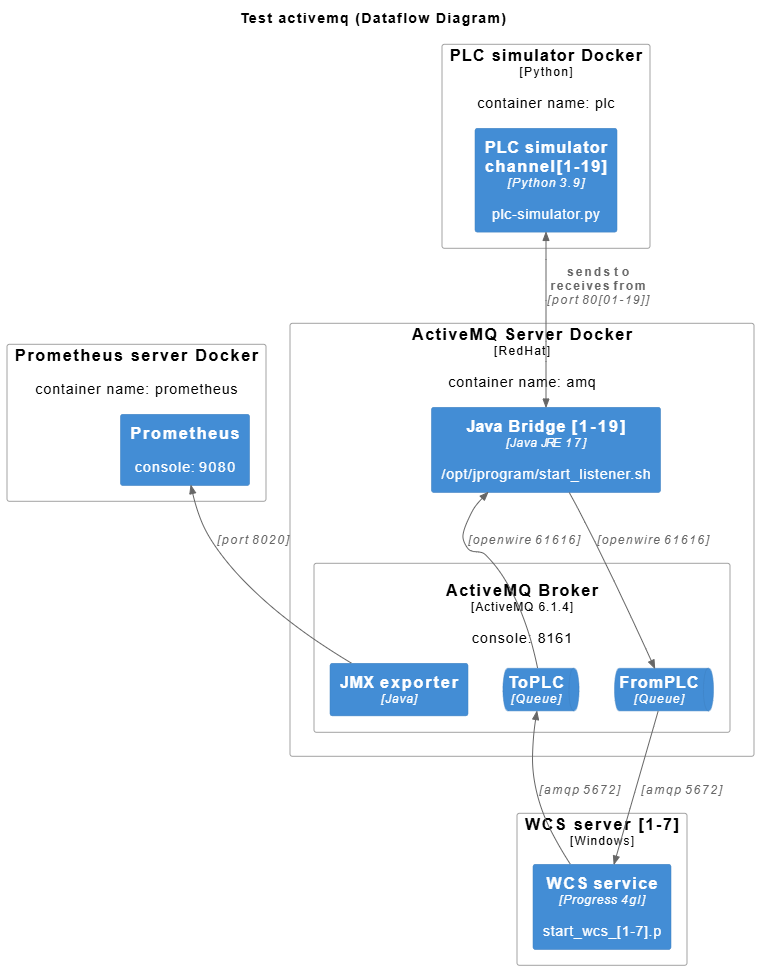
\includegraphics[width=.95\textwidth]{img/test_amq_dataflow.png}
  \caption{\label{fig:test_amq_dataflow}Dataflow test AMQ}
\end{figure}

\subsubsection{Installatie}
Het installeren van dit systeem wordt duidelijk uitgelegd in de officiële documentatie van Apache ActiveMQ.
Configuratie moet aangepast worden in ``activemq.xml'' (\hyperref[listing:configxml_activemq]{zie bijlage: Configuratie}) om de service toegankelijk te maken voor externe services.
Daarnaast moet het bestand ``setenv'' (\hyperref[listing:configxml_activemq]{zie bijlage: Configuratie}) aangepast worden om de metrics via ``jmx\_exporter'' beschikbaar te maken.

\subsubsection{Integratie}
Het WCS-script kan via poort 5672 een AMQP-verbinding tot stand brengen met de ActiveMQ-server.
De Java-listeners op die server zijn een aparte service en maken gebruik van een JMS-library. 
Daarom is het optimaal om via het OpenWire-protocol te verbinden op poort 61616. 
OpenWire is een native protocol van Apache ActiveMQ en wordt vaak gebruikt voor eenvoudige toepassingen, zoals deze, in een Java-omgeving.
\\\\
Om de simulatie zo realistisch mogelijk te maken, zijn er twee queues opgezet. 
Berichten afkomstig van de PLC worden via de gebruikte poort, via de Java-listener naar de queue gestuurd en krijgen daarbij een property genaamd kanaal.
Dankzij deze property kunnen de berichten eenvoudig worden gefilterd op kanaal. 
\\\\
Voor monitoring wordt de ``jmx\_exporter'' gebruikt, waarmee de metrics beschikbaar worden gesteld aan externe software zoals Prometheus. 
Deze monitoringdata kan benaderd worden via een zelf te configureren poort, in dit geval poort 8020.

\subsubsection{Performantie}
In deze test worden 19 PLC connecties gemaakt met de Java listeners die elk per 0.1 seconde een bericht versturen naar de  ``FromPLC'' queue.
Hierdoor worden meer dan 1680 berichten per minuut gesimuleerd en wordt er voldaan aan de minimale vereisten op gebied van performantie.
Het opmeten van deze test wordt verdeeld in twee categorieën, enqueued- en dequeued messages.
Om correct de throughput te meten moeten we beide categorieën meten omdat dit de volledige transactie representeert. 
\\\\
Volgende grafiek bevestigd dat er per minuut meer dan 1680 berichten kan geplaatst worden op de twee queues:
\begin{figure}[h!]
  \centering
  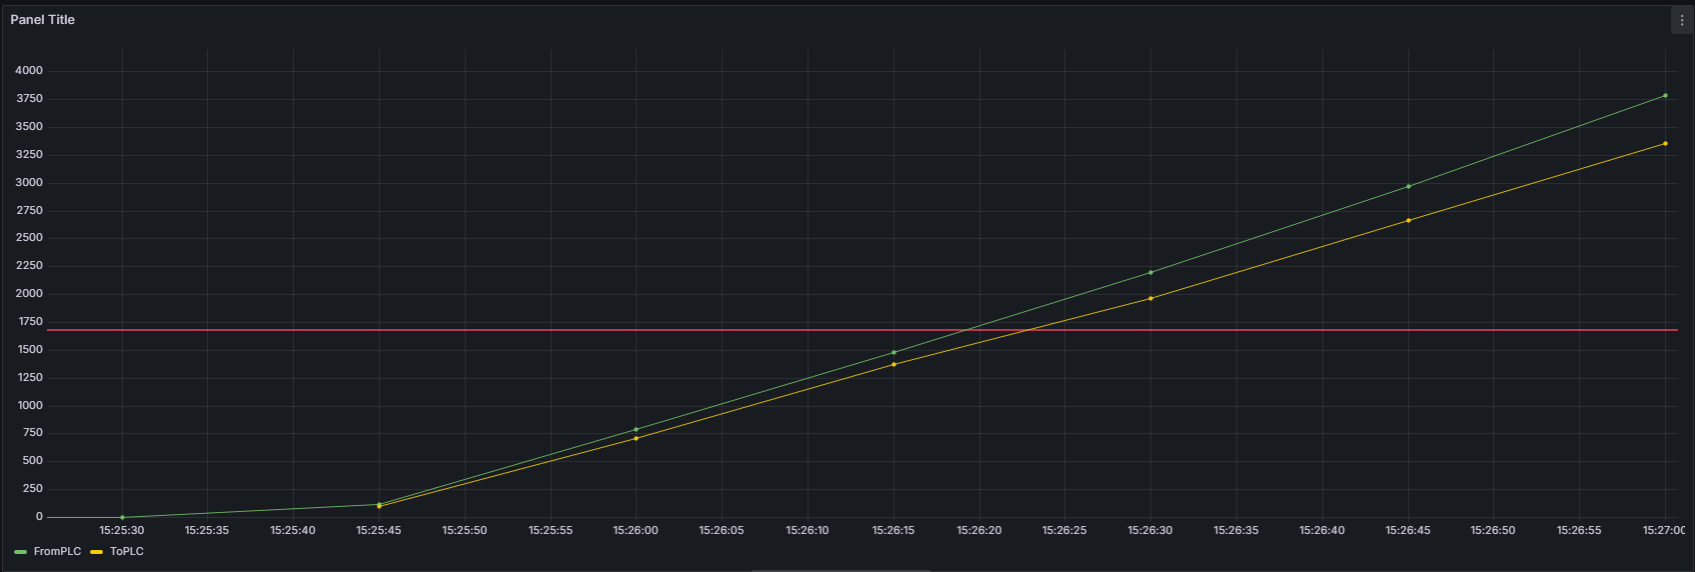
\includegraphics[width=.95\textwidth]{img/amq-enqueue-count.png}
  \caption{\label{fig:amq_enqueue_count}Enqueue ActiveMQ}
\end{figure}
\newpage
Zoals de grafiek laat zien kan de message broker meer dan 1680 berichten naar de consumer versturen van iedere queue binnen één minuut.
\begin{figure}[h!]
  \centering
  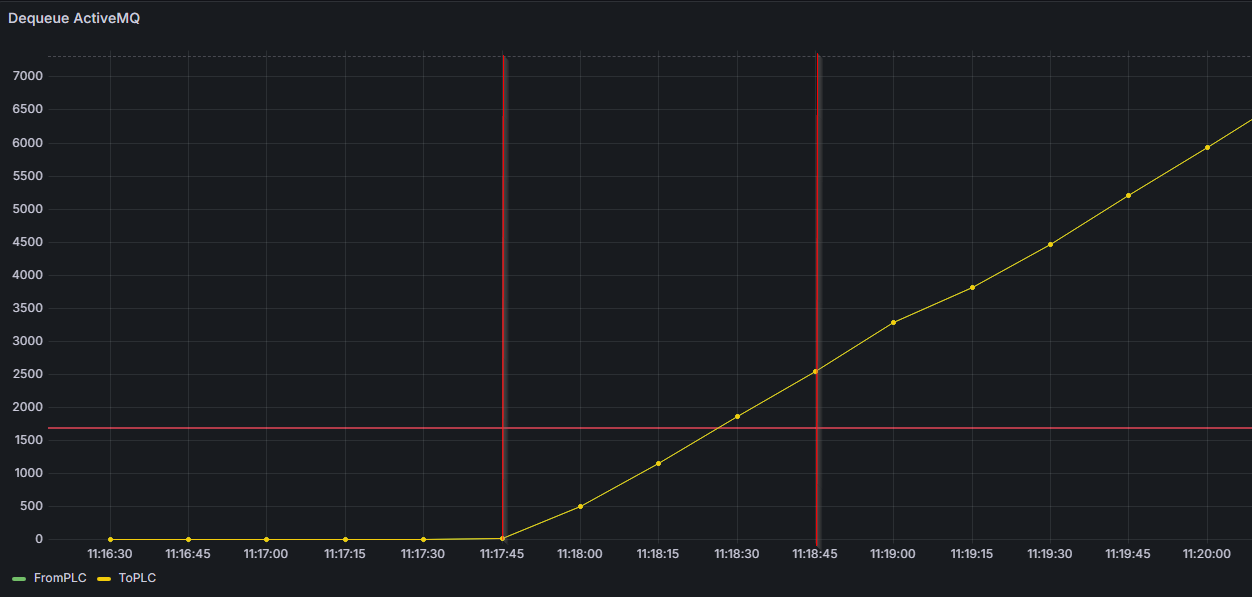
\includegraphics[width=.95\textwidth]{img/amq-dequeue-count.png}
  \caption{\label{fig:amq_dequeue_count}Dequeue ActiveMQ}
\end{figure}

De volgende grafiek toont het aantal berichten dat binnen één minuut is ontvangen. 
Dit resultaat is, net als bij de vorige test, afhankelijk van het systeem waarop wordt getest. 
Productieomgevingen leveren doorgaans betere prestaties dan de testomgeving.
\begin{figure}[h!]
  \centering
  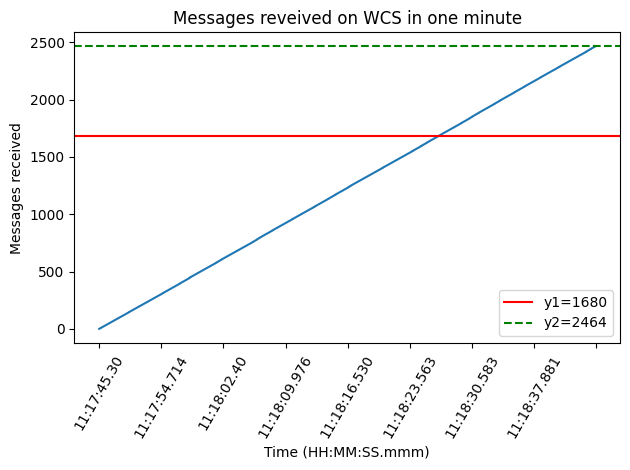
\includegraphics[width=.95\textwidth]{img/amq_received_wcs.png}
  \caption{\label{fig:amq_received_wcs}ActiveMQ berichten ontvangen door WCS}
\end{figure}

\subsubsection{Samenvatting}
De installatie en integratie kunnen worden uitgevoerd zonder al te complexe aanpassingen, 
wat het proces gebruiksvriendelijk en eenvoudig maakt.
Monitoring is eenvoudig en gemakkelijk toegankelijk. 
Een mooie extra is de admin console die beschikbaar is via ``http://localhost:8161/admin'', waar de metrics kunnen worden geraadpleegd.
Wat betreft prestaties voldoet dit product aan de verwachtingen omdat het meer dan 1680 berichten binnen één minuut kan verwerken via twee queues.

\newpage
\subsection{Test RabbitMQ}
In deze test werd opnieuw een Docker container gemaakt met een RedHat OS instantie, waarop RabbitMQ 
werd geïnstalleerd via een \hyperref[listing:docker_rabbitmq]{DockerFile}.
\\\\
Overzicht infrastructuur:
\begin{figure}[!h]
  \centering
  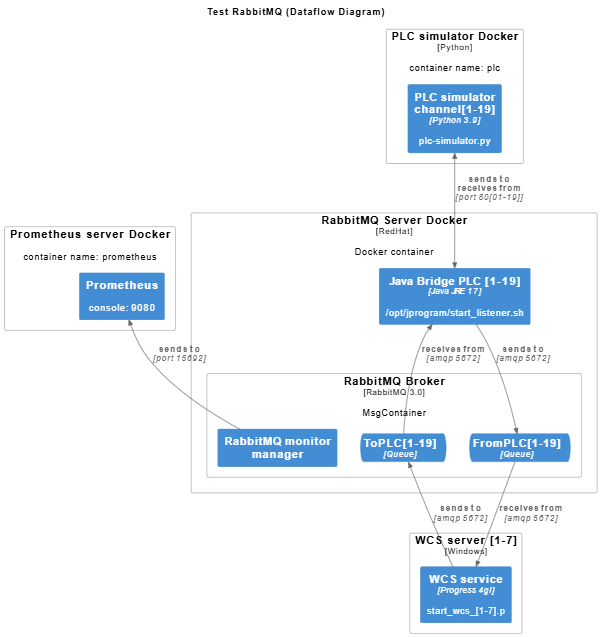
\includegraphics[width=.95\textwidth]{img/test-rabbitmq-dataflow.png}
  \caption{\label{fig:test_rabbitmq_dataflow}Dataflow test RabbitMQ}
\end{figure}

\subsubsection{Installatie}
Deze software heeft een zeer uitgebreide documentatie op de officiële site waardoor het gemakkelijk te installeren is.
RabbitMQ vereist officiële repositories voor uitbreidingen, Erlang runtime en GPG-sleutels om de installatie te verifiëren.
Er is geen configuratie bestand voorzien tijdens de installatie waardoor de originele settings van kracht zijn.
Om deze settings aan te passen is er in de documentatie een voorbeeld configuratiebestand (\hyperref[sec:config_rabbitmq]{zie bijlage: configuratie}) voorzien.
De basis configuratie kan met minimale aanpassingen een werkende messaging broker tot stand brengen.
Omdat de configuratie uitgebreid is, kan deze technologie voldoen aan complexe opstellingen.

\subsubsection{Integratie}
Om de Java listeners en het WCS te laten communiceren met de message broker, is er gekozen voor het AMQP protocol via poort 5672.
Monitoring voor Prometheus is voorzien in het RabbitMQ management pakket en is bereikbaar via ``http://localhost:15672/''.
Omdat er geen filtering mogelijk is moet er voor ieder kanaal een queue voorzien worden en wijken we af van de opzet van het huidige systeem.
Hierdoor zijn er 38 queues nodig, 19 voor de FromPLC berichten en 19 voor de ToPLC berichten.
\\\\
Berichten kunnen enkel verstuurd worden als binaire data waardoor de inhoud van een bericht eerst moet omgezet worden naar een binary array door de producer.
Ook na het consumeren van een bericht moet deze eerst omgezet worden van binaire data naar het string datatype.

\subsubsection{Performantie}
In deze test worden opnieuw 19 socket connecties gemaakt door het plc script met de Java listeners die elk per 0.1 seconde een bericht versturen naar de relevante queue.
Hierdoor worden meer dan 1680 berichten per minuut verstuurd om te kunnen voldoen aan de minimale vereisten op gebied van performantie.
Het opmeten van deze test wordt verdeeld in twee categorieën, enqueued- en dequeued messages.
Het verschil met vorige test is dat er hier meerdere queues zijn, 19 voor de FromPLC en 19 voor de ToPLC. 

\begin{figure}[h!]
  \centering
  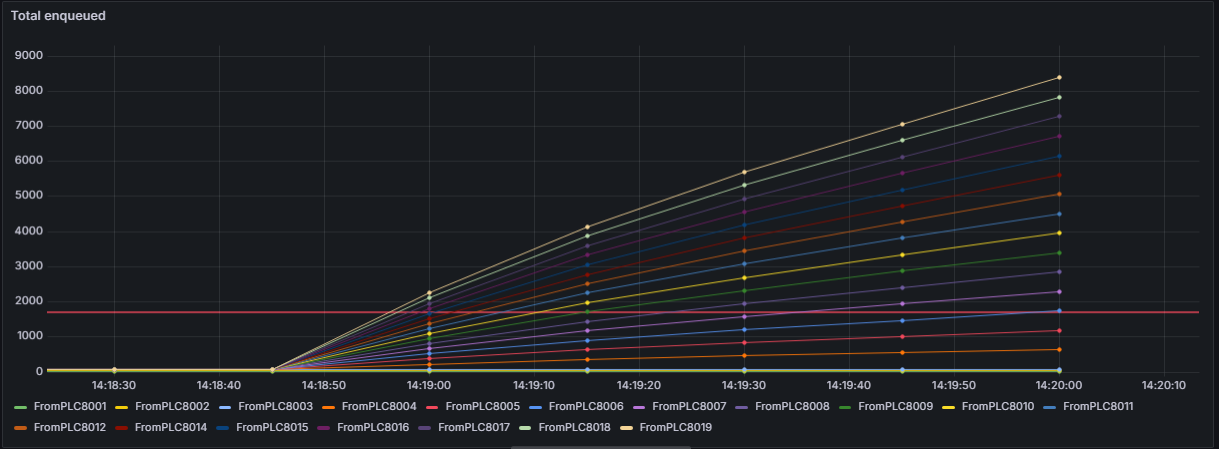
\includegraphics[width=.95\textwidth]{img/rabbitmq-enqueue-count-FromPLC.png}
  \caption{\label{fig:rabbitmq_enqueue_fromplc_count}RabbitMQ enqueue FromPLC}
\end{figure}

\begin{figure}[h!]
  \centering
  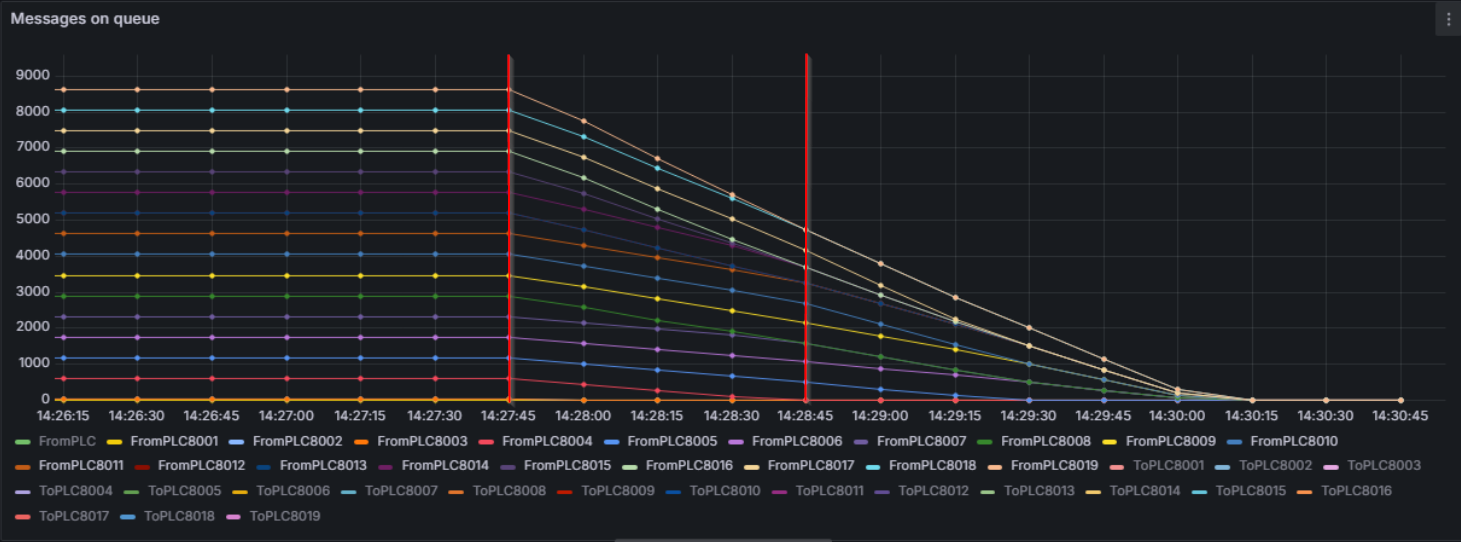
\includegraphics[width=.95\textwidth]{img/rabbitmq-dequeue-count-FromPLC.png}
  \caption{\label{fig:rabbitmq_dequeue_fromplc_count}RabbitMQ dequeue FromPLC}
\end{figure}

\begin{figure}[h!]
  \centering
  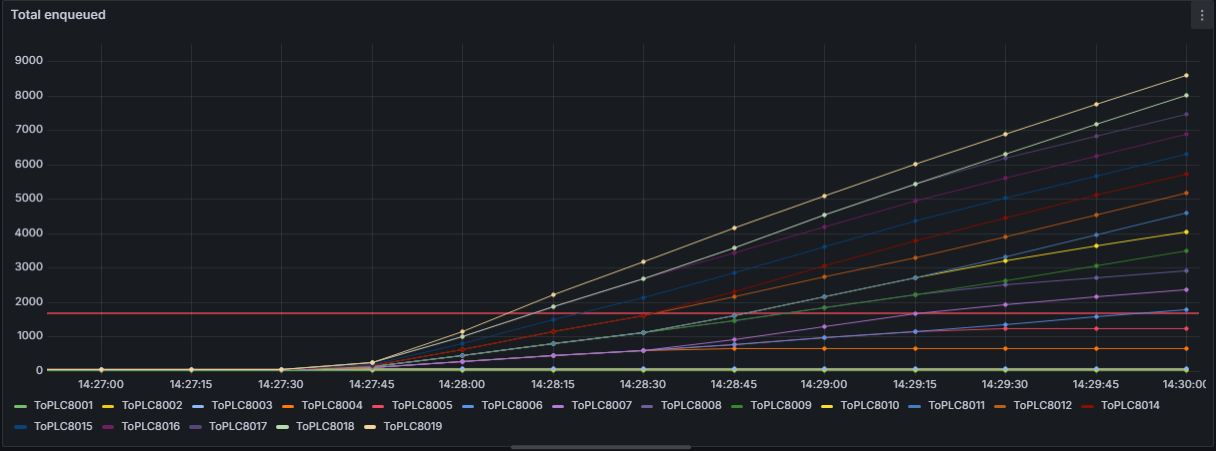
\includegraphics[width=.95\textwidth]{img/rabbitmq-enqueue-count-ToPLC.png}
  \caption{\label{fig:rabbitmq_enqueue_toplc_count}RabbitMQ enqueue ToPLC}
\end{figure}

\begin{figure}[h!]
  \centering
  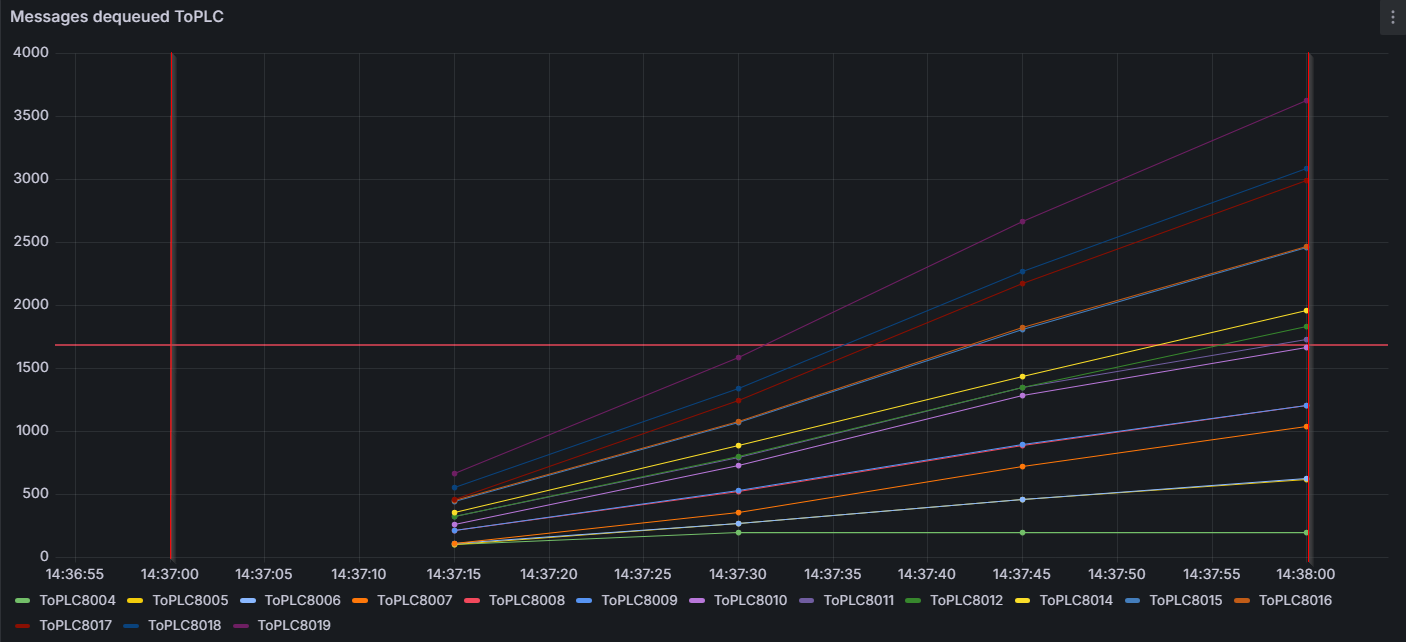
\includegraphics[width=.95\textwidth]{img/rabbitmq-dequeue-count-ToPLC.png}
  \caption{\label{fig:fig:rabbitmq_dequeue_fromplc_count}RabbitMQ dequeue ToPLC}
\end{figure}

\subsubsection{Samenvatting}
RabbitMQ lijkt een goede oplossing dat compatibel is met het huidige systeem, 
maar heeft wel wat aanpassingen nodig omdat filtering niet kan toegepast worden.
Om dit product te gebruiken moet er voor ieder kanaal een aparte queue voorzien worden.
Daarnaast moeten berichten ook omgezet worden en verstuurd worden als binaire data.
\newpage

\subsection{Test Artemis}
In deze test wordt ook een \hyperref[listing:docker_artemis]{Dockerfile} gebruikt voor de installatie.
Overzicht van de infrastructuur:
\begin{figure}[h!]
  \centering
  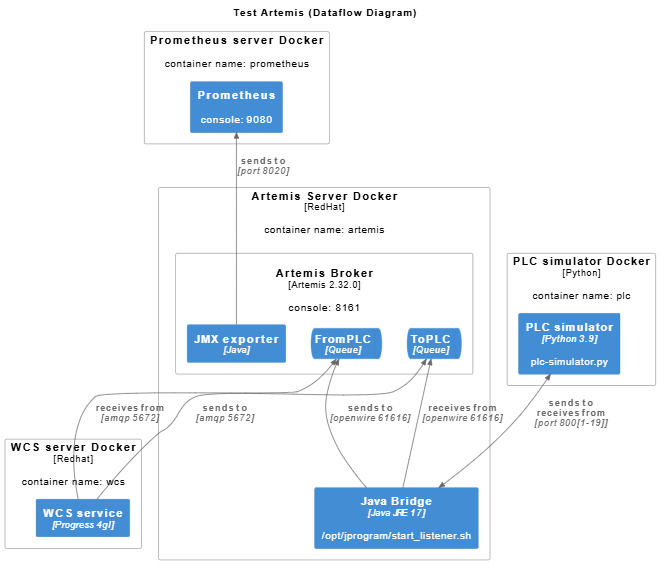
\includegraphics[width=.95\textwidth]{img/test-artemis-dataflow.png}
  \caption{\label{fig:test_artemis_dataflow}Dataflow test Artemis}
\end{figure}

\subsubsection{Installatie}
Het installeren van dit systeem wordt net zoals de andere technologieën duidelijk uitgelegd in de officiële documentatie van Apache.
Configuratie moet hier niet aangepast worden in ``broker.xml'' (\hyperref[listing:broker_artemis]{zie bijlage: configuratie Artemis}) om de service toegankelijk te maken voor externe services.
Artemis kan verschillende broker instanties opstarten binnen dezelfde JVM, in tegenstelling tot bijvoorbeeld ActiveMQ, dat slechts één instantie kan starten.

\subsubsection{Integratie}
Om de metrics aan te bieden kan je een artemis-prometheus plugin downloaden en toevoegen in de installatie.
Hiervoor moet de ``broker.xml'' aangepast worden met het toevoegen van de metrics plugin.
deze maakt de metrics toegankelijk via een webpagina.
Hiervoor moet de plugin gecompileerd worden zodat de ``metrics.war'' in de web folder van actieve broker kan geplaatst worden.
Om de webpagina beschikbaar te maken moet de ``bootstrap.xml'' (\hyperref[listing:bootstrap_artemis]{zie bijlage: configuratie Artemis}) aangepast worden.

\subsubsection{Performantie}
In deze test worden 19 PLC connecties gemaakt met de Java listeners die elk per 0.1 seconde een bericht versturen naar de ``FromPLC'' queue.
Hierdoor worden meer dan 1680 berichten per minuut verstuurd en wordt er voldaan aan de minimale vereisten op gebied van performantie.
Het opmeten van deze test wordt verdeeld in twee categorieën, enqueued- en dequeued messages.
Om correct de throughput te meten moeten we beide categorieën meten omdat dit de volledige transactie representeert. 
\\\\
Volgende grafiek geeft weer hoeveel berichten er per minuut verzonden kunnen worden naar de message queue.
\begin{figure}[h!]
  \centering
  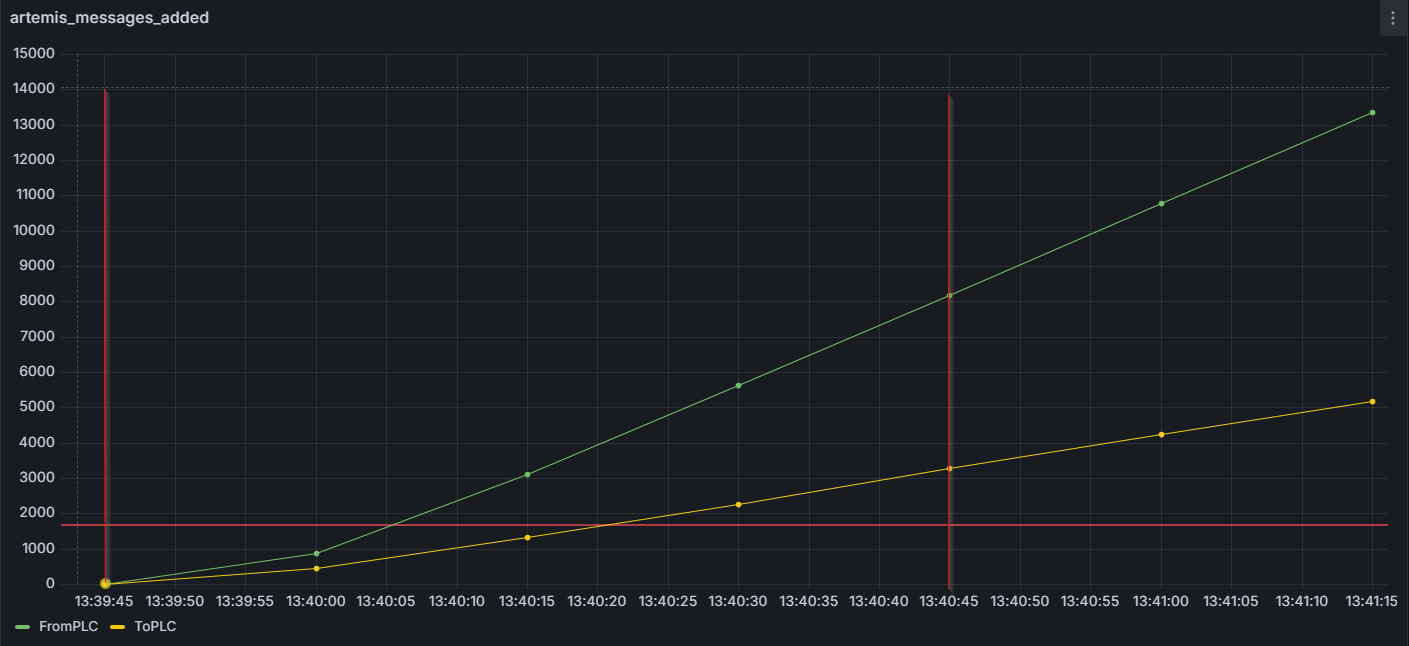
\includegraphics[width=.95\textwidth]{img/artemis-enqueue-count.png}
  \caption{\label{fig:artemis_enqueue_count}Enqueue Artemis}
\end{figure}

\begin{figure}[h!]
  \centering
  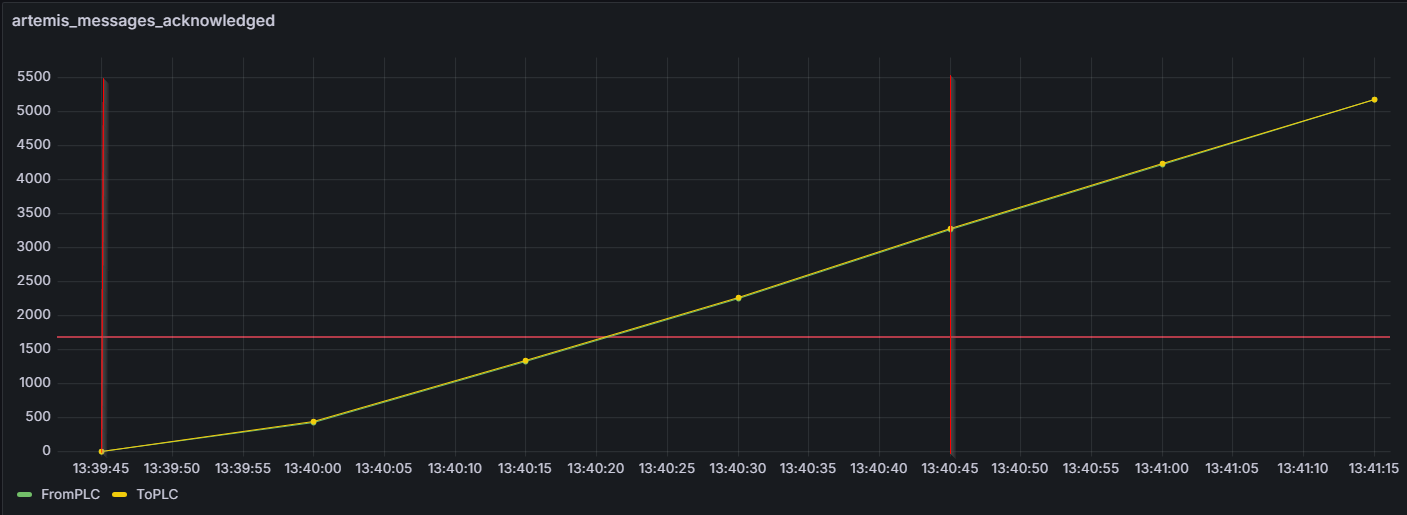
\includegraphics[width=.95\textwidth]{img/artemis-dequeue-count.png}
  \caption{\label{fig:artemis_dequeue_count}Dequeue Artemis}
\end{figure}

\subsubsection{Samenvatting}
De installatie en integratie kunnen worden uitgevoerd zonder al te complexe aanpassingen, 
wat het proces gebruiksvriendelijk en eenvoudig maakt.
Het voorzien van monitoring is evenals eenvoudig en gemakkelijk toegankelijk. 
De admin console is beschikbaar via ``http://localhost:8161'' en is gebruiksvriendelijk en uitgebreider dan de admin console van ActiveMQ Classic.
Wat betreft prestaties voldoet dit product aan de verwachtingen omdat het meer dan 1680 PLC berichten binnen één minuut kan verwerken.